

\subsection{Miscellaneous Options}
\label{pgfplots:misc}

\begin{pgfplotskey}{disablelogfilter=\mchoice{true,false} (initally false, default true)}
Disables numerical evaluation of $\log(x)$ in \TeX. If you specify this option, any plot coordinates and tick positions must be provided as $\log(x)$ instead of $x$. This may be faster and -- possibly -- more accurate than the numerical log. The current implementation of $\log(x)$ normalizes~$x$ to $m\cdot 10^e$ and computes
\[ \log(x) = \log(m) + e \log(10) \]
where $y = \log(m)$ is computed with a newton method applied to $\exp(y) - m$. The normalization involves string parsing without \TeX-registers. You can savely evaluate $\log(1\cdot 10^{-7})$ although \TeX-registers would produce an underflow for such small numbers. 
\end{pgfplotskey}

\label{sec:disabledatascaling}%
\begin{pgfplotskey}{disabledatascaling=\mchoice{true,false} (initally false, default true)}
\index{Accuracy!Data Transformation}%
\index{Errors!dimension too large}%
Disables internal re-scaling of input data. Normally, every input data like plot coordinates, tick positions or whatever, are parsed without using \TeX's limited number precision. Then, a transformation like 
	\[ T(x) = 10^{q-m} \cdot x - a \]
is applied to every input coordinate/position where $m$ is ``the order of $x$'' base~$10$. Example: $x=1234 = 1.234\cdot 10^3$ has order~$m=4$ while $x=0.001234 = 1.234\cdot 10^{-3}$ has order $m=-2$. The parameter~$q$ is the order of the axis' width/height.

The \textbf{effect} of the transformation is that your plot coordinates can be of \emph{arbitrary magnitude} like $0.0000001$ and $0.0000004$. For these two coordinates, \PGFPlots\ will use 100pt and 400pt internally. The transformation is quit fast since it relies only on period shifts. This scaling allows precision beyond \TeX's capabilities.
%\footnote{Please note that while plot coordinates can be of quite large magnitude like $10^12$ or $10^{-9}$, \PGFPlots\ still uses \TeX-registers internally (the math parser of \PGF). If your axis interval is $[1234567.8, 1234567.9]$ or something like that, }.

The option ``|disabledatascaling|'' disables this data transformation. This has two consequences: first, coordinate expressions like \parg{{\normalfont\texttt{axis cs:}}x,y} have the same effect like \parg{x,y}, no re-scaling is applied. Second, coordinates are restricted to what \TeX\ can handle\footnote{Please note that the axis' scaling requires to compute $1/( x_\text{max} - x_{\text{min}} )$. The option \protect\pgfmanualpdfref{disabledatascaling}{\texttt{disabledatascaling}} may lead to overflow or underflow in this context, so use it with care! Normally, the data scale transformation avoids this problem.}.

So far, the data scale transformation applies only to normal axis (logarithmic scales do not need it). 
\end{pgfplotskey}


\begin{pgfplotskey}{execute at begin plot=\marg{commands}}
This axis option allows to invoke \marg{commands} at the beginning of each |\addplot| command. The argument \marg{commands} can be any \TeX\ content.

You may use this in conjunction with |x filter=...| to reset any counters or whatever. An example would be to change every $4$th coordinate.
\end{pgfplotskey}

\begin{pgfplotskey}{execute at end plot=\marg{commands}}
This axis option allows to invoke \marg{commands} after each |\addplot| command. The argument \marg{commands} can be any \TeX\ content.
\end{pgfplotskey}

\begin{pgfplotskey}{forget plot=\marg{true,false} (initially false)}
\label{pgfplots:forgetplot}
	Allows to include plots which are not remembered for legend entries, which do not increase the number of plots and which are not considered for cycle lists.

	A forgotten plot can be some sort of decoration which has a separate style and does not influence the axis state, although it is processed as any other plot.
	Provide this option to |\addplot| as in the following example.
\begin{codeexample}[]
\begin{tikzpicture}
	\begin{loglogaxis}[
		% some descriptions:
		table/x=Basis,
		table/y={L2/r},
		xlabel=Degrees of Freedom,
		ylabel=relative Error,
		title=New Experiments (old in gray),
		legend entries={$e_1$,$e_2$,$e_3$}
	]
	\addplot[black!15,forget plot] 
		table {plotdata/oldexperiment1.dat};
	\addplot[black!15,forget plot] 
		table {plotdata/oldexperiment2.dat};
	\addplot[black!15,forget plot] 
		table {plotdata/oldexperiment3.dat};
	\addplot table {plotdata/newexperiment1.dat};
	\addplot table {plotdata/newexperiment2.dat};
	\addplot table {plotdata/newexperiment3.dat};
	\end{loglogaxis}
\end{tikzpicture}
\end{codeexample}
	Since forgotten plots won't increase the plot index, they will use the same |cycle list| entry as following plots. 

	The style |every forget plot| can be used to configure styles for each such plot:
\begin{codeexample}[]
\begin{tikzpicture}
    \begin{loglogaxis}[
		forget plot style={opacity=0.2},
		% same as above:
        table/x=Basis,
        table/y={L2/r},
        xlabel=Degrees of Freedom,
        ylabel=relative Error,
        title=New Experiments (old in transparent),
        legend entries={$e_1$,$e_2$,$e_3$},
    ]
	\foreach \exp in {1,2,3} {
      \addplot+[forget plot]
          table {plotdata/oldexperiment\exp.dat};
      \addplot table {plotdata/newexperiment\exp.dat};
	}
    \end{loglogaxis}
\end{tikzpicture}	
\end{codeexample}
	\noindent Here, the |\addplot+| command means we are using the same |cycle list| as the following plot and |forget plot style| modifies |every forget style| and yields transparency of the ``old experiments''.
	
	Please note that |every plot no |\meta{index} styles are not applicable here.

	A forgotten plot will be stacked normally if |stack plots| is enabled!
\end{pgfplotskey}

\begin{pgfplotscodekey}{before end axis}
Allows to insert \marg{commands} just before the axis is ended. This option takes effect inside of the clipped area.
\begin{codeexample}[]
\pgfplotsset{every axis/.append style={
	before end axis/.code={
		\fill[red] (axis cs:1,10) circle(5pt);
		\node at (axis cs:-4,10) 
			{\large This text has been inserted 
			 using \texttt{before end axis}.};
	}}}
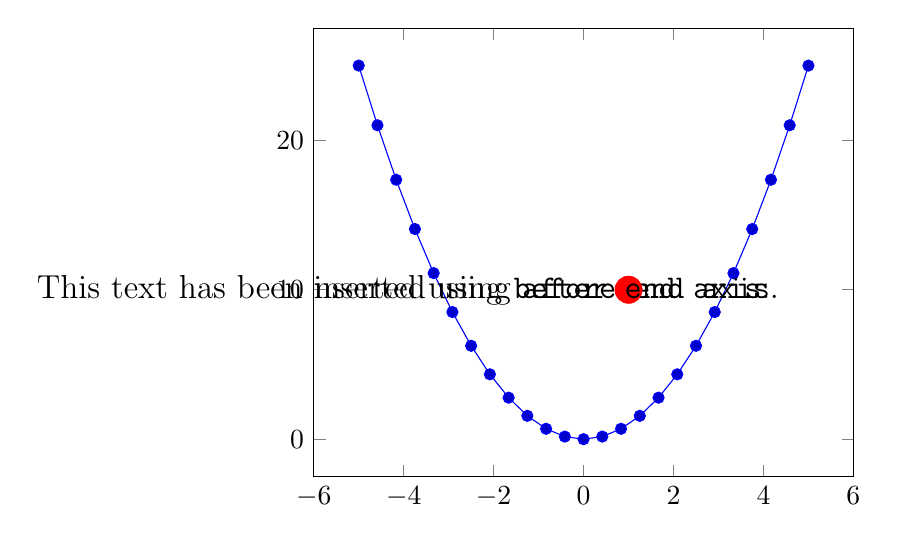
\begin{tikzpicture}
	\begin{axis}
	\addplot {x^2};
	\end{axis}
\end{tikzpicture}
\end{codeexample}
\end{pgfplotscodekey}

\begin{pgfplotscodekey}{after end axis}
Allows to insert \marg{commands} right after the end of the clipped drawing commands. While |befor end axis| has the same effect as if \marg{commands} had been placed inside of your axis, |after end axis| allows to access axis coordinates without being clipped.
\begin{codeexample}[]
\pgfplotsset{every axis/.append style={
	after end axis/.code={
		\fill[red] (axis cs:1,10) circle(5pt);
		\node at (axis cs:-4,10) 
			{\large This text has been inserted using \texttt{after end axis}.};
	}}}
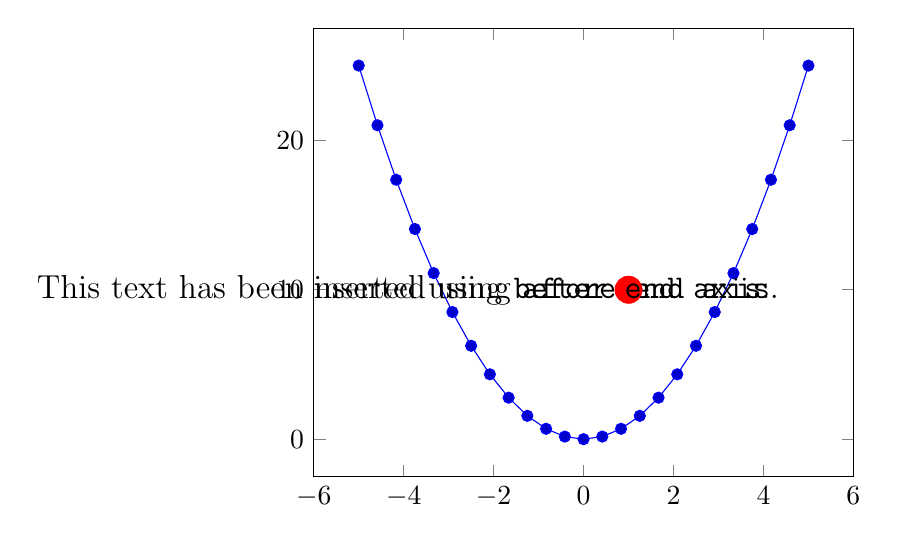
\begin{tikzpicture}
	\begin{axis}
	\addplot {x^2};
	\end{axis}
\end{tikzpicture}
\end{codeexample}
\end{pgfplotscodekey}

\begin{pgfplotskey}{clip marker paths=\mchoice{true,false} (initially false)}
	The initial choice |clip marker paths=false| causes markers to be drawn \emph{after} the clipped region. Only their positions will be clipped. As a consequence, markers will be drawn completely, or not at all. The value |clip marker paths=true| is here for backwards compatibility: it does not introduce special marker treatment, so markers may be drawn partially if they are close to the clipping boundary\footnote{Please note that clipped marker paths may be slightly faster during \TeX\ compilation.}.
\end{pgfplotskey}

\begin{pgfplotskey}{clip=\mchoice{true,false} (initially true)}
	Whether any paths inside an axis shall be clipped.
\end{pgfplotskey}

\begin{pgfplotskey}{axis on top=\mchoice{true,false} (initially false)}
	If set to |true|, axis lines, ticks, tick labels and grid lines will be drawn on top of plot graphics.
\begin{codeexample}[]
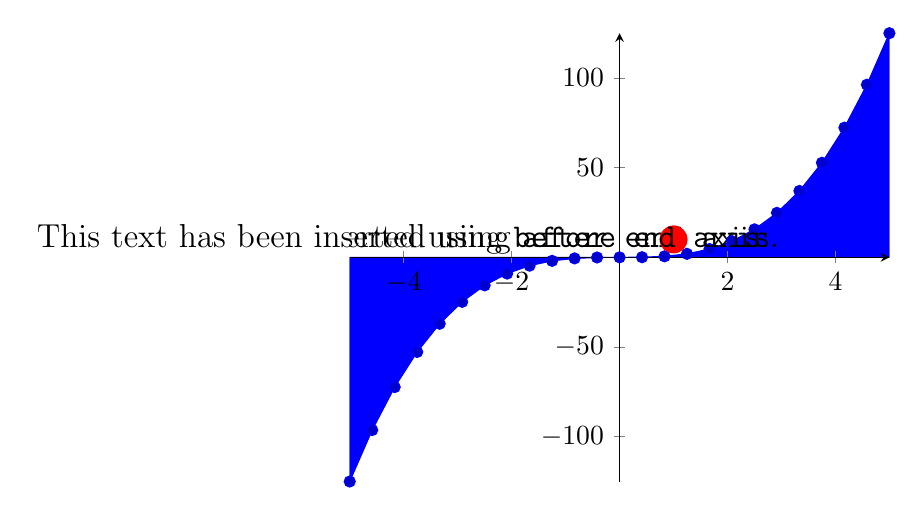
\begin{tikzpicture}
    \begin{axis}[
		axis on top=true,
		axis x line=middle,
		axis y line=middle]
    \addplot+[fill] {x^3} \closedcycle;
    \end{axis}
\end{tikzpicture}
\end{codeexample}

\begin{codeexample}[]
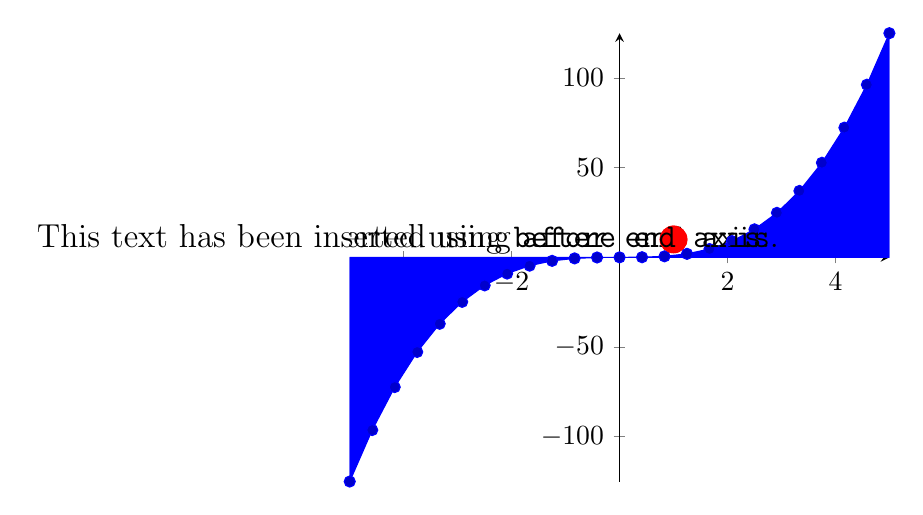
\begin{tikzpicture}
    \begin{axis}[
		axis on top=false,
		axis x line=middle,
		axis y line=middle]
    \addplot+[fill] {x^3} \closedcycle;
    \end{axis}
\end{tikzpicture}
\end{codeexample}
Please note that this feature does not affect plot marks. I think it looks unfamiliar if plot marks are crossed by axis descriptions.
\end{pgfplotskey}


\begin{pgfplotskeylist}{%
	visualization depends on=\meta{\textbackslash macro} (initially empty),%
	visualization depends on=\meta{expression}\texttt{\textbackslash as}\meta{\textbackslash macro} (initially empty),
	visualization depends on=\texttt{value}\meta{content}\texttt{\textbackslash as}\meta{\textbackslash macro} (initially empty)}
	Allows to communicate data to \PGFPlots\ which is essential to perform the visualization although \PGFPlots\ isn't aware of it.

	Suppose you want a scatter plot, which depends on the $(x,y)$ coordinates, the |point meta| data to draw individual colors and furthermore data which influences the |mark size|. Thus, you need a total of~$4$ coordinates for every data point, although \PGFPlots\ supports only $3$ in its initial configuration.
	
	Before we actually come to the main point of the problem, we'll talk about how to get a scatter plot which has individual colors \emph{and} individual sizes. It is not sufficient to set |mark size| alone, since |mark size| is evaluated only once, before markers are processed (the same holds for |every mark|). Thus, we can use |scatter| combined with

	|scatter/@pre marker code/.append style={/tikz/mark size=\perpointmarksize}|.

	\noindent The |@pre marker code| is installed for every marker of a scatter plot individually. Now, we come to the problem as such: where can we get the value for |mark size|, in our case called |\perpointmarksize|?
	
	A solution is |visualization depends on| (using the second input syntax at this point):
\begin{codeexample}[]
\begin{tikzpicture}
\begin{axis}
	\addplot+[
		scatter,
		scatter src=y,
		samples=40,
		visualization depends on=
			{5*cos(deg(x)) \as \perpointmarksize},
		scatter/@pre marker code/.append style=
			{/tikz/mark size=\perpointmarksize}
	]
		{sin(deg(x))};
\end{axis}
\end{tikzpicture}
\end{codeexample}
	
	Here, we define |\perpointmarksize| as |5*cos(deg(x))|. The expression will be evaluated together with all other coordinates. Thus, everything which is available during the survey phase can be used here. This includes the final coordinates |x|, |y|, |z|; the constant |meta| expands to the current per point meta data. Furthermore, |\thisrow|\marg{colname} expands to the value of a table column.

	The command |visualization depends on| evaluates and remembers every value in internal data structures. The remembered value is then available as \meta{\textbackslash macro} during the visualization phase. In our example, the |@pre marker code| is evaluated during the visualization phase and applies |mark size=5*cos(deg(x))|.
	
	The first syntax, |visualization depends on=|\meta{\textbackslash macro}, tells \PGFPlots\ to use an already defined \meta{\textbackslash macro}. The second syntax with \meta{content}|\as|\meta{\textbackslash macro} provides also the value.

	There can be more than one |visualization depends on| phrase.

	In case the stored value is not of numerical type\footnote{Or if it is just a constant and you'd like to improve speed.}, you can use the prefix `|value|' before the argument, i.e.

	|visualization depends on=value |\meta{\textbackslash macro} or

	|visualization depends on=value |\meta{content}|\as |\meta{\textbackslash macro}.

	Such a value will be expanded and stored, but not parsed as number (at least not by \PGFPlots).
\end{pgfplotskeylist}

\begin{key}{/pgf/fpu=\marg{true,false} (initially true)}
\index{Precision}
	This key activates or deactivates the floating point unit. If it is disabled (|false|), the core \PGF\ math engine written by Mark Wibrow and Till Tantau will be used for |plot expression|.
	However, this engine has been written to produce graphics and is not suitable for scientific computing. It is limited to fixed point numbers in the range $\pm 16384.00000$.

	If the |fpu| is enabled (|true|, the initial configuration) the high-precision floating point library of \PGF\ written by Christian Feuers\"anger will be used. It offers the full range of IEEE double precision computing in \TeX. This FPU is also part of \PGFPlotstable, and it is activated by default for |create col/expr| and all other predefined mathematical methods.

	Use
\begin{codeexample}[code only]
\pgfkeys{/pgf/fpu=false}
\end{codeexample}
	\noindent in order to de-activate the extended precision. If you prefer using the |fp| (fixed point) package, possibly combined with Mark Wibrows corresponding \PGF\ library, the |fpu| will be deactivated automatically. Please note, however, that |fp| has a smaller data range (about $\pm 10^{17}$) and may be slower.
\end{key}
